%  !TeX  root  =  user_guide.tex

\chapter{Panoramica sulle caratteristiche}\label{feature_glance}

% when the revision of a section has been finalized, 
% comment out the following line:
%\updatedisclaimer

Dopo un primo sguardo e una semplice sessione d'esempio nella Sezione \ref{label_getstarted},
questo capitolo fornisce una panoramica maggiormente dettagliata delle caratteristiche di QGIS. 
Molte delle caratteristiche presentate nei successivi capitoli saranno spiegate
e descritte nelle apposite sezioni del manuale.

\section{Avvio e chiusura di QGIS}\label{label_startinqgis}

Nella sezione \ref{samplesession} abbiamo già  imparato come avviare QGIS. Ripeteremo 
questa operazione qui per mostrare come QGIS fornisca ulteriori opzioni all'avvio da riga di comando. 

\begin{itemize}
\item \nix{Assumendo che QGIS sia installato nel vostro PATH, lo si può avviare  
digitando: \usertext{qgis}  al prompt dei comandi o facendo doppio click sul
collegamento all'applicazione (o shortcut) sul desktop o nel menu delle applicazioni.} 
\item \win{Avviare QGIS usando il menu Avvio (Start) o il collegamento sul desktop, 
o facendo doppio click su un progetto QGIS precedentemente salvato.}
\item \osx{Fare doppio click sull'icona QGIS nella cartella Applicazioni (Applications). Se si vuole avviare QGIS
in una shell, eseguire /percorso-installazione-eseguibile/Contents/MacOS/Qgis.}
\end{itemize} 

Per uscire da QGIS, cliccare sul menu \{\nix{}\win{File} \osx{QGIS}\} \arrow Esci,
o usare la scorciatoia da tastiera \keystroke{Ctrl+Q}.

\subsection{Opzioni da linea di comando}\index{opzioni da linea di comando}
\label{label_commandline}

\nix QGIS supporta un certo numero di opzioni se avviato da riga di comando.
Per avere una lista delle opzioni possibili, digitare \usertext{qgis ---help} al prompt dei comandi.
La sintassi d'uso di QGIS è la seguente:

\small
\begin{verbatim}
qgis --help
Quantum GIS - 1.7.0-Wroclaw 'Wroclaw' (exported)
Quantum GIS (QGIS) is a viewer for spatial data sets, including
raster and vector data.
Usage: qgis [options] [FILES]
  options:
        [--snapshot filename]           emit snapshot of loaded datasets to given file
        [--width width]                 width of snapshot to emit
        [--height height]               height of snapshot to emit
        [--lang language]               use language for interface text
        [--project projectfile]         load the given QGIS project
        [--extent xmin,ymin,xmax,ymax]  set initial map extent
        [--nologo]                      hide splash screen
        [--noplugins]                   don't restore plugins on startup
        [--optionspath path]            use the given QSettings path
        [--configpath path]             use the given path for all user configuration
        [--help]                        this text

  FILES:
    Files specified on the command line can include rasters,
    vectors, and QGIS project files (.qgs):
     1. Rasters - Supported formats include GeoTiff, DEM
        and others supported by GDAL
     2. Vectors - Supported formats include ESRI Shapefiles
        and others supported by OGR and PostgreSQL layers using
        the PostGIS extension
\end{verbatim}
\normalsize

\begin{Tip} \caption{\textsc{Esempio di utilizzo delle opzioni da riga di comando}}
QGIS può essere avviato specificando uno o più file di dati da riga di comando.
Per esempio, assunto che ci si trovi nella directory 
qgis\_sample\_data, si può avviare QGIS con un layer vettoriale e un file raster inserendo il seguente comando:
\usertext{qgis ./raster/landcover.img ./gml/lakes.gml}
\end{Tip}

\minisec{Opzione da linea di comando \usertext{---snapshot}}
L'opzione consente di creare uno snapshot in formato PNG della vista corrente.
Questo può essere utile quando si hanno molti progetti e si vogliono
generare schermate dai propri dati.

Il file PNG generato ha una risoluzione di 800x600 pixels. Questa può essere adattata
usando gli argomenti da riga di comando \usertext{---width} e \usertext{---height}. 
Dopo l'opzione \usertext{---snapshot} può essere specificato il nome del file con cui si vuole salvare l'immagine.

\minisec{Opzione da linea di comando \usertext{---lang}}
L'interfaccia di QGIS si presenta nella lingua definita dalle impostazioni di localizzazione di sistema.
Se si desidera l'interfaccia in un'altra lingua, lo si può specificare all'avvio. Ad esempio:
\usertext{---lang=en}
fa sì che QGIS si avvii localizzato in inglese.
Un elenco delle lingue supportate è disponibile all'indirizzo
\url{http://www.qgis.org/wiki/GUI_Translation_Progress} 

\minisec{Opzione da linea di comando \usertext{---project}}
E' possibile avviare QGIS anche con un file di progetto. Basta semplicemente
aggiungere l'opzione da riga di comando \usertext{---project} seguita dal percorso e dal nome
del progetto e QGIS si aprirà caricando tutti i layer indicati nel file specificato.

\minisec{Opzione da linea di comando \usertext{---extent}}
Per fare sì che QGIS si avvii visualizzando una specifica porzione di mappa, è necessario specificare 
i limiti dell'estensione (bounding box) che si intende visualizzare secondo il seguente ordine, con ogni 
valore separato da virgole:
\begin{verbatim}
--extent xmin,ymin,xmax,ymax
\end{verbatim}

\minisec{Opzione da linea di comando \usertext{---nologo}}
Questa opzione nasconde lo splash screen quando QGIS viene avviato.

\minisec{Opzione da linea di comando \usertext{---noplugins}}
Se si verificano problemi con i plugin all'avvio di QGIS, è possibile evitare di caricarli. Saranno comunque disponibili in seguito nel Gestore plugin.

\minisec{Opzione da linea di comando \usertext{---optionspath}}
Potreste avere più di una configurazione e con questa opzione potete decidere quale usare al momento di avviare QGIS. 
Si veda la Sezione \ref{subsec:gui_options} per controllare dove il vostro sistema operativo salva i file d'impostazione. Al momento non c'è modo di specificare in quale file salvare le impostazioni, per cui potete creare una copia del file di impostazione e rinominarlo.

\minisec{Opzione da linea di comando \usertext{---configpath}}
Questa opzione è simile alla precedente, ma in più sovrascrive il percorso di default (~/.qgis) per le configurazioni utente e forza anche QSettings ad usare questo percorso. Questo permette all'utente, ad esempio, di portare l'installazione di QGIS su una flash drive (es. una chiave USB) insieme a tutti i plugin ed impostazioni.

\section{Interfaccia grafica di QGIS}\index{finestra principale}
\label{label_qgismainwindow}

All'avvio di QGIS viene visualizzata l'interfaccia grafica riprodotta dalla seguente immagine  
(i numeri da 1 a 6 negli ovali gialli fanno riferimento alle sei principali aree dell'interfaccia 
come di seguito specificato):

\begin{figure}[ht]
   \centering
    \includegraphics[clip=true, width=12cm]{startup}
    \caption{Interfaccia grafica di QGIS con i dati campione dell'Alaska \nixcaption} \label{fig:startup}
\end{figure}

\textbf{Nota:} L'aspetto delle finestre (barra del titolo, ecc.) può apparire diverso a seconda 
del sistema operativo e del gestore di finestre utilizzato.\\

L'interfaccia di QGIS è divisa in sei aree:

\begin{tabular}{p{5cm} p{5cm}}
%\centering
1. Barra dei Menu & 4. Vista Mappa \\
2. Barra degli Strumenti & 5. Panoramica \\
3. Legenda & 6. Barra di Stato \\
\end{tabular}

Le sei componenti dell'interfaccia di QGIS sono descritte con maggior dettaglio
nelle sezioni seguenti. Due ulteriori sezioni descriveranno le scorciatoie da 
tastiera e la guida contestuale.

% \newpage

\subsection{Barra dei menu}\label{label_menubar}
\index{barra menu}

La barra dei menu fornisce accesso alle varie caratteristiche di QGIS utilizzando 
un menu gerarchico standard. Le voci gerarchicamente più elevate e una sintesi 
di alcune opzioni di menu sono elencate di seguito, assieme alle icone degli 
strumenti corrispondenti così come appaiono nella barra degli strumenti ed alle 
scorciatoie da tastiera usate per richiamarli.\footnote{Le scorciatoie da tastiera 
possono essere configurate manualmente (quelle presentate in questa sezione sono quelle predefinite), 
usando lo strumento Configura le scorciatoie nel menu Modifica.} Sebbene molte voci di menu abbiano 
uno strumento corrispondente e viceversa, i menu non sono organizzati esattamente come le barre degli strumenti.
La barra degli strumenti che contiene la voce descritta è indicata dopo ogni voce di 
menu con l'aspetto di una casella di controllo (checkbox). Per ulteriori informazioni su 
strumenti e barre degli strumenti si veda la Sezione \ref{label_toolbars}.

\begin{tabbing}
\hspace{5.5cm}\=\hspace{3cm}\=\hspace{3.5cm}\= \kill
\hspace{1cm} Voce di Menu \> Scorciatoia \> Riferimento \> Barra degli strumenti\\
\end{tabbing}

\begin{itemize}
\item \mainmenuopt{File}
\begin{tabbing}
\hspace{4.5cm}\=\hspace{3cm}\=\hspace{3.5cm}\= \kill
\dropmenuopttwo{mActionFileNew}{Nuovo progetto}
	\> \keystroke{Ctrl+N}
	\> sezione \ref{sec:projects}
	\> \dropmenucheck{File} \\
\dropmenuopttwo{mActionFileOpen}{Apri progetto}
	\> \keystroke{Ctrl+O}
	\> sezione \ref{sec:projects}
	\> \dropmenucheck{File} \\
\dropmenuopt{Apri progetti recenti}
	\>
	\> sezione \ref{sec:projects} \\
\dropmenuopttwo{mActionFileSave}{Salva progetto}
	\> \keystroke{Ctrl+S}
	\> sezione \ref{sec:projects}
	\> \dropmenucheck{File} \\
\dropmenuopttwo{mActionFileSaveAs}{Salva progetto con nome}
	\> \keystroke{Ctrl+Shift+S}
    \> sezione \ref{sec:projects}
	\> \dropmenucheck{File} \\
\dropmenuopttwo{mActionSaveMapAsImage}{Salva come immagine}
	\>
	\> sezione \ref{sec:output} \\
\dropmenuopttwo{mActionNewComposer}{Nuova composizione di stampa}
        \> \keystroke{Ctrl+P}
        \> sezione \ref{label_printcomposer}
        \> \dropmenucheck{File} \\
\dropmenuopttwo{mActionComposerManager}{Gestore di stampe}
	\> 
	\> sezione \ref{label_printcomposer}
	\> \dropmenucheck{File} \\
\dropmenuopt{Stampe}
	\>
	\> sezione \ref{label_printcomposer} \\
\dropmenuopttwo{mActionFileExit}{Esci} 
	\> \keystroke{Ctrl+Q} \\
\end{tabbing}

\item \mainmenuopt{Modifica}
\begin{tabbing}
\hspace{4.5cm}\=\hspace{3cm}\=\hspace{3.5cm}\= \kill
\dropmenuopttwo{mActionUndo}{Annulla}
        \> \keystroke{Ctrl+Z}
        \> sezione \ref{sec:advanced_edit}
        \> \dropmenucheck{Digitalizzazione avanzata} \\
\dropmenuopttwo{mActionRedo}{Ripristina}
        \> \keystroke{Ctrl+Shift+Z}
        \> sezione \ref{sec:advanced_edit}
        \> \dropmenucheck{Digitalizzazione avanzata} \\
\dropmenuopttwo{mActionEditCut}{Taglia geometria}
	\> \keystroke{Ctrl+X}
	\> sezione \ref{sec:edit_existing_layer}
	\> \dropmenucheck{Digitalizzazione} \\
\dropmenuopttwo{mActionEditCopy}{Copia elementi}
	\> \keystroke{Ctrl+C}
	\> sezione \ref{sec:edit_existing_layer}
	\> \dropmenucheck{Digitalizzazione} \\
\dropmenuopttwo{mActionEditPaste}{Incolla elementi}
	\> \keystroke{Ctrl+V}
	\> sezione \ref{sec:edit_existing_layer}
	\> \dropmenucheck{Digitalizzazione} \\
\dropmenuopttwo{mActionEditPaste}{Muovi elemento/i}
        \>
        \> sezione \ref{sec:edit_existing_layer}
        \> \dropmenucheck{Digitalizzazione} \\
\dropmenuopttwo{mActionDeleteSelected}{Elimina il selezionato}
        \>
        \> sezione \ref{sec:edit_existing_layer}
        \> \dropmenucheck{Digitalizzazione} \\
\dropmenuopttwo{mActionSimplify}{Semplifica geometria}
        \>
        \> sezione \ref{sec:advanced_edit}
        \> \dropmenucheck{Digitalizzazione avanzata} \\
\dropmenuopttwo{mActionAddRing}{Aggiungi buco}
        \>
        \> sezione \ref{sec:advanced_edit}
        \> \dropmenucheck{Digitalizzazione avanzata} \\
\dropmenuopttwo{mActionAddIsland}{Aggiungi una parte}
        \>
        \> sezione \ref{sec:advanced_edit}
        \> \dropmenucheck{Digitalizzazione avanzata} \\
\dropmenuopttwo{mActionDeleteRing}{Elimina buco}
        \>
        \> sezione \ref{sec:advanced_edit}
        \> \dropmenucheck{Digitalizzazione avanzata} \\
\dropmenuopttwo{mActionDeletePart}{Elimina parte}
        \>
        \> sezione \ref{sec:advanced_edit}
        \> \dropmenucheck{Digitalizzazione avanzata} \\
\dropmenuopttwo{mActionReshape}{Modifica la forma}
        \>
        \> sezione \ref{sec:advanced_edit}
        \> \dropmenucheck{Digitalizzazione avanzata} \\
\dropmenuopttwo{mActionSplitFeatures}{Spezza elemento}
        \>
        \> sezione \ref{sec:advanced_edit}
        \> \dropmenucheck{Digitalizzazione avanzata} \\
\dropmenuopttwo{mActionMergeFeatures}{Unisci le geometrie selezionate}
        \>
        \> sezione \ref{sec:advanced_edit}
        \> \dropmenucheck{Digitalizzazione avanzata} \\
\dropmenuopttwo{mActionMergeFeatures}{Unisci gli attributi delle geometrie selezionate}
        \>
        \> sezione \ref{sec:advanced_edit}
        \> \dropmenucheck{Digitalizzazione avanzata} \\
\dropmenuopttwo{mActionNodeTool}{Strumento vertici}
        \>
        \> sezione \ref{sec:edit_existing_layer}
        \> \dropmenucheck{Digitalizzazione} \\
\dropmenuopttwo{mActionRotatePointSymbols}{Ruota i simboli per i punti}
        \>
        \> sezione \ref{sec:advanced_edit}
        \> \dropmenucheck{Digitalizzazione avanzata} \\
\end{tabbing}

Quando si attiva la modalità \toolbtntwo{mActionToggleEditing}{Modifica} per un layer, ulteriori voci vengono aggiunte nel menu \mainmenuopt{Modifica} in funzione del tipo di geometria (punto, linea o poligono). \\

\begin{tabbing}
\hspace{4.5cm}\=\hspace{3cm}\=\hspace{3.5cm}\= \kill
\dropmenuopttwo{mActionCapturePoint}{Inserisci punto}
        \>
        \> sezione \ref{sec:edit_existing_layer}
        \> \dropmenucheck{Digitalizzazione} \\
\dropmenuopttwo{mActionCaptureLine}{Inserisci linea}
        \>
        \> sezione \ref{sec:edit_existing_layer}
        \> \dropmenucheck{Digitalizzazione} \\
\dropmenuopttwo{mActionCapturePolygon}{Inserisci poligono}
        \>
        \> sezione \ref{sec:edit_existing_layer}
        \> \dropmenucheck{Digitalizzazione} \\
\end{tabbing}

\item \mainmenuopt{Visualizza}
\begin{tabbing}
\hspace{4.5cm}\=\hspace{3cm}\=\hspace{3.5cm}\= \kill
\dropmenuopttwo{mActionPan}{Sposta mappa}
	\>
	\> \> \dropmenucheck{Navigazione mappa} \\
\dropmenuopttwo{mActionZoomIn}{Ingrandisci}
	\> \keystroke{Ctrl++}
	\> \> \dropmenucheck{Navigazione mappa} \\
\dropmenuopttwo{mActionZoomOut}{Rimpicciolisci}
	\> \keystroke{Ctrl+-}
	\> \> \dropmenucheck{Navigazione mappa} \\
\dropmenuopt{Seleziona}
	\> 
	\> sezione \ref{sec:selection} 
	\> \dropmenucheck{Attributi} \\
\dropmenuopttwo{mActionIdentify}{Informazioni elementi}
	\> \keystroke{Ctrl-Shift-I}
	\> \> \dropmenucheck{Attributi} \\	
\dropmenuopt{Misura}
	\> 
	\> sezione \ref{sec:measure}
	\> \dropmenucheck{Attributi} \\
\dropmenuopttwo{mActionOpenTable}{Zoom completo}
	\> \keystroke{Ctrl-Shift-F}
	\> \> \dropmenucheck{Navigazione mappa} \\
\dropmenuopttwo{mActionZoomToLayer}{Zoom sul layer}
	\>
	\> \> \dropmenucheck{Navigazione mappa} \\
\dropmenuopttwo{mActionZoomToSelected}{Zoom alla selezione}
	\> \keystroke{Ctrl+J}
	\> \> \dropmenucheck{Navigazione mappa} \\
\dropmenuopttwo{mActionZoomLast}{Ultimo zoom}
	\>
	\> \> \dropmenucheck{Navigazione mappa} \\
\dropmenuopttwo{mActionZoomNext}{Zoom successivo}
	\>
	\> \> \dropmenucheck{Navigazione mappa} \\
\dropmenuopt{Zoom alla dimensione corrente}
	\>
	\> \>  \\	
\dropmenuopttwo{mActionMapTips}{Suggerimenti mappa}
	\>
	\> \> \dropmenucheck{Attributi} \\
\dropmenuopttwo{mActionNewBookmark}{Nuovo segnalibro}
	\> \keystroke{Ctrl+B}
	\> sezione \ref{sec:bookmarks} 
\> \dropmenucheck{Attributi} \\
\dropmenuopttwo{mActionShowBookmarks}{Mostra segnalibri}
	\> \keystroke{Ctrl-Shift-B}
	\> sezione \ref{sec:bookmarks} 
	\> \dropmenucheck{Attributi} \\
\dropmenuopttwo{mActionDraw}{Aggiorna}
	\> \keystroke{Ctrl+R}
	\> \> \dropmenucheck{Navigazione mappa} \\
\mainmenuopt{Slider per la scala delle tiles}
	\>
	\> sezione \ref{sec:tilesets}
	\> \dropmenucheck{Scala delle tiles} \\
\mainmenuopt{Tracciamento GPS in tempo reale}
	\>
	\> sezione \ref{sec:gpstracking}
	\> \dropmenucheck{Informazioni sul GPS} \\
\dropmenuopt{Pannelli}
	\>
	\>
	\\
\dropmenuopt{Barre degli strumenti}
	\>
	\>
	\\
\mainmenuopt{Schermo Intero}
	\>\keystroke{Ctrl-F}
	\>
	\\
\end{tabbing}

\item \mainmenuopt{Layer}
\begin{tabbing}
\hspace{5cm}\=\hspace{3cm}\=\hspace{3.5cm}\= \kill
\dropmenuopt{Nuovo}
	\>
	\> sezione \ref{sec:create shape}
	\> \dropmenucheck{Gestione layer} \\
\dropmenuopttwo{mActionAddNonDbLayer}{Aggiungi vettore}       
	\> \keystroke{Ctrl+Shift+V}
	\>          	
	sezione \ref{label_workingvector}
	\> \dropmenucheck{Gestione layer} \\
\dropmenuopttwo{mActionAddRasterLayer}{Aggiungi raster}       
	\> \keystroke{Ctrl+Shift+R}
	\>          	
	sezione \ref{label_raster}
	\> \dropmenucheck{Gestione layer} \\
\dropmenuopttwo{mActionAddLayer}{Aggiungi vettore PostGIS}      
	\> \keystroke{Ctrl+Shift+D}
	\>          	
	sezione \ref{label_postgis}
        \> \dropmenucheck{Gestione layer} \\
\dropmenuopttwo{mActionAddSpatiaLiteLayer}{Aggiungi un layer SpatiaLite}
        \> \keystroke{Ctrl+Shift+L}
        \>
        sezione \ref{label_spatialite}
	\> \dropmenucheck{Gestione layer} \\
\dropmenuopttwo{mActionAddWmsLayer}{Aggiungi layer WMS}          
	\> \keystroke{Ctrl+Shift+W}
	\>          	
	sezione \ref{sec:ogc-wms}
	\> \dropmenucheck{Gestione layer} \\
\dropmenuopttwo{mActionOpenTable}{Apri tabella attributi}
	\> \>
	\> \dropmenucheck{Attributi} \\
\dropmenuopttwo{mActionFileSave}{Salva modifiche}
        \> \>
        \> \dropmenucheck{Digitalizzazione} \\
\dropmenuopttwo{mActionToggleEditing}{Modifica}
	\> \>
	\> \dropmenucheck{Digitalizzazione} \\
\mainmenuopt{Salva con nome...}
	\\
\mainmenuopt{Salva selezione come vettore...}
	\> 
	\> sezione \ref{sec:attribute table}
	\> \\	
\dropmenuopttwo{mActionRemoveLayer}{Elimina layer}
	\> \keystroke{Ctrl+D}
	\>
	\> \\
\mainmenuopt{Imposta SR del/i layer}
	\> \keystroke{Ctrl+Shift+C}
	\>
	\> \\
\mainmenuopt{Imposta SR progetto dal layer}
	\\
\mainmenuopt{Proprietà}
	\\
\mainmenuopt{Query...}
	\\
\dropmenuopttwo{labeling}{Etichettatura}
	\>
	\>
	\\
\dropmenuopttwo{mActionInOverview}{Aggiungi alla panoramica}
	\> \keystroke{Ctrl+Shift+O}
	\>
	\> 
    \dropmenucheck{Gestione layer} \\
\dropmenuopttwo{mActionAddAllToOverview}{Aggiungi tutto alla panoramica}
	\>
	\>
	\\
\dropmenuopttwo{mActionRemoveAllFromOverview}{Rimuovi tutto dalla panoramica}
	\>
	\>
	\\
\dropmenuopttwo{mActionShowAllLayers}{Mostra tutti i layer}
	\> \keystroke{Ctrl+Shift+U}
	\>
	\> \dropmenucheck{Gestione layer} \\
\dropmenuopttwo{mActionHideAllLayers}{Nascondi tutti i layer}
	\> \keystroke{Ctrl+Shift+H}
	\>
	\> \dropmenucheck{Gestione layer} \\
\end{tabbing}	

\item \mainmenuopt{Impostazioni}
\begin{tabbing}
\hspace{5cm}\=\hspace{3cm}\=\hspace{3.5cm}\= \kill
\dropmenuopttwo{mActionProjectProperties}{Proprietà progetto}  
	\> \keystroke{Ctrl-Shift-P}
	\> sezione \ref{sec:projects}
	\\
\dropmenuopttwo{mActionCustomProjection}{SR personalizzato}   
	\> \> sezione \ref{sec:customprojections}
	\\
\dropmenuopt{Gestore di stili}
        \>
        \>
        \\
\dropmenuopttwo{mActionOptions}{Configura scorciatoie}
        \>
        \>
        \\
\dropmenuopttwo{mActionOptions}{Opzioni}             
	\> \> sezione \ref{subsec:gui_options}
	\\
\dropmenuopt{Opzioni di snap}
        \>
        \>
        \\
\end{tabbing}

\item \mainmenuopt{Plugins} - (Ulteriori voci di menu vengono aggiunte quando si installano e caricano nuovi plugin.)
\begin{tabbing}
\hspace{4.5cm}\=\hspace{3cm}\=\hspace{3.5cm}\= \kill
\dropmenuopttwo{mActionShowPluginManager}{Gestione Plugins}          	 
	\> \> sezione \ref{sec:managing_plugins} \dropmenucheck{Plugin}
	\\
\mainmenuopt{Console python}
        \> \>
        \\
\end{tabbing}        	

\item \mainmenuopt{Raster}
\begin{tabbing}
\hspace{5cm}\=\hspace{3cm}\=\hspace{3.5cm}\= \kill
\mainmenuopt{Calcolatore raster}
        \>
        \> sezione \ref{sec:raster_calc}
        \>  \\
\end{tabbing}

\item \mainmenuopt{Guida}
\begin{tabbing}
\hspace{5cm}\=\hspace{3cm}\=\hspace{3.5cm}\= \kill
\dropmenuopttwo{mActionHelpContents}{Contenuti della guida}
	\> \keystroke{F1}
	\>           	
	\> \dropmenucheck{Guida}\\
\mainmenuopt{Documentazione sulle API}
        \>
        \> 
        \>  \\
\dropmenuopttwo{mActionQgisHomePage}{Home Page di QGIS}
	\> \keystroke{Ctrl+H}
	\>          	
	\\
\dropmenuopttwo{mActionCheckQgisVersion}{Controlla la versione di QGIS}
	\\
\dropmenuopttwo{mActionHelpAbout}{Informazioni}
	\\
\dropmenuopttwo{mActionHelpSponsors}{Sponsor QGIS}
	\\
\end{tabbing}
\end{itemize}

%See Appendix \ref{app_menu} for complete descriptions of the menu items.

\subsection{Barre degli strumenti}\label{label_toolbars}
\index{barre degli strumenti}

Le barre degli strumenti forniscono accesso alla maggior parte delle medesime funzioni presenti nei menu,
oltre a funzioni addizionali per interagire con la mappa. Ogni oggetto della barra degli strumenti
ha un aiuto a comparsa (popup). Lasciando il cursore del mouse sopra l'icona verrà 
visualizzata una breve descrizione della funzione fornita da quello strumento.

Ogni barra può essere spostata secondo le preferenze personali. Inoltre ognuna di esse
può essere disattivata dal menu contestuale cliccando con il tasto destro del mouse
sulla barra degli strumenti.

\begin{Tip}
\caption{\textsc{Ripristinare le barre degli strumenti}} \index{disposizione!barre degli strumenti}
Se avete accidentalmente disattivato tutte le barre strumenti,
potete ripristinarle dalla voce di menu \mainmenuopt{Visualizza} \arrow \dropmenuopt{Barre degli strumenti}.
\end{Tip}

\subsection{Legenda}\label{label_legend}
\index{legenda}

L'area di legenda è usata per impostare la visibilità  e l'ordine di sovrapposizione dei layer:
i layer in cima alla legenda coprono nella mappa quelli sottostanti (z-ordering).
La casella di controllo in ogni legenda può essere usata per attivare/disattivare la 
visibilità  di un layer.\index{layer!visibilità}
Un layer può essere selezionato e trascinato in modo da modificarne la visibilità (z-ordering).

I layer nell'area di legenda possono essere organizzati in gruppi. A tal fine cliccare con il tasto destro del mouse nell'area di legenda e selezionare \dropmenuopt{Aggiungi gruppo}, quindi assegnare un nome al gruppo e premere il tasto 
\keystroke{Invio}. Ora è possibile cliccare e trascinare layer esistenti all'interno del gruppo: se si aggiungono nuovi layer al progetto, mentre un gruppo è selezionato, gli stessi verranno assegnati al gruppo. 
Per rimuovere un layer da un gruppo è possibile cliccare e trascinare il layer al di fuori dello stesso o in alternativa cliccare con il tasto destro del mouse sul layer e selezionare \dropmenuopt{Muovi fuori dal gruppo}.

I gruppi possono essere nidificati all'interno di altri gruppi. La casella di controllo di un gruppo può essere usata per mostrare/nascondere tutti i layer del gruppo con un singolo clic.

Il contenuto del menu contestuale varia a seconda che si faccia click col tasto destro del mouse
su un layer raster o vettoriale. Per i layer vettoriali di GRASS la voce di menu \dropmenuopt{Modifica}
non è abilitata. Si veda la sezione \ref{grass_digitising} per informazioni su come modificare layer vettoriali GRASS. 

\begin{itemize}

\item \textbf{Menu contestuale per i raster}
\begin{itemize}
\item \dropmenuopt{Zoom all'estensione del layer}
\item \dropmenuopt{Zoom alla scala migliore (100\%)}
\item \dropmenuopt{Aggiungi alla panoramica}
\item \dropmenuopt{Rimuovi}
\item \dropmenuopt{Imposta il SR del layer}
\item \dropmenuopt{Imposta il SR del del progetto dal layer}
\item \dropmenuopt{Proprietà}
\item \dropmenuopt{Rinomina}
\item \dropmenuopt{Aggiungi gruppo}
\item \dropmenuopt{Espandi tutto}
\item \dropmenuopt{Comprimi tutto}
\end{itemize}

\item \textbf{Menu contestuale per i vettori}
\begin{itemize}
\item \dropmenuopt{Zoom all'estensione del layer}
\item \dropmenuopt{Aggiungi alla panoramica}
\item \dropmenuopt{Rimuovi}
\item \dropmenuopt{Imposta il SR del layer}
\item \dropmenuopt{Imposta il SR del del progetto dal layer}
\item \dropmenuopt{Apri tabella attributi}
\item \dropmenuopt{Modifica (non disponibile per i layer GRASS)}
\item \dropmenuopt{Salva con nome}
\item \dropmenuopt{Salva la selezione con nome}
\item \dropmenuopt{Query}
\item \dropmenuopt{Mostra totale oggetti}
\item \dropmenuopt{Proprietà}
\item \dropmenuopt{Muovi oggetto fuori dal gruppo}
\item \dropmenuopt{Rinomina}
\item \dropmenuopt{Aggiungi gruppo}
\item \dropmenuopt{Espandi tutto}
\item \dropmenuopt{Comprimi tutto}
\end{itemize}

\item \textbf{Menu contestuale per i gruppi di layer} 
\begin{itemize}
\item \dropmenuopt{Zoom al gruppo}
\item \dropmenuopt{Rimuovi}
\item \dropmenuopt{Imposta il SR di gruppo}
\item \dropmenuopt{Rinomina}
\item \dropmenuopt{Aggiungi gruppo}
\item \dropmenuopt{Espandi tutto}
\item \dropmenuopt{Comprimi tutto}
\end{itemize}

\end{itemize}

È possibile selezionare più di un layer o gruppo allo stesso tempo
tenendo premuto il tasto \keystroke{CTRL} e selezionando con il tasto sinistro del mouse. 
Tutti i layer così selezionati possono essere spostati contemporaneamente in un nuovo gruppo, oppure essere cancellati premendo il tasto \keystroke{CTRL-D}.

\subsection{Vista mappa}\label{label_mapview}
\index{mappa!vista}

Questa è l'area in cui le mappe vengono visualizzate. La mappa visualizzata in questa finestra sarà
il risultato dei layer vettoriali e/o raster che si è scelto di caricare (vedere le sezioni che seguono
per ulteriori informazioni su come caricare i layer). La zona di visualizzazione della mappa può
essere modificata (spostando la messa a fuoco dell'esposizione della mappa ad un'altra regione) ed
è possibile effettuare operazioni di zoom in ed out (+ e -). Varie altre operazioni sono descritte nella
sezione relativa alla barra dei menu. La vista nell'area di mappa e la legenda sono strettamente
legate l'un l'altra: le mappe che vengono visualizzate riflettono i cambiamenti fatti nella area
della legenda.  

\begin{Tip}\caption{\textsc{Zoom in e zoom out con la rotella del mouse}}\index{zoom!mouse wheel}
Per le operazioni di zoom è anche possibile utilizzare la rotella del mouse. 
Posizionando il puntatore del mouse nell'area di visualizzazione delle mappe si aumenta
lo zoom girando la rotella verso lo schermo, lo si riduce girandola nel verso contrario. La posizione del puntatore costituisce il centro per l'ingrandimento. Il comportamento della funzione di zoom con la rotella del mouse può essere
regolata dalla scheda \tab{Strumenti di mappa} sotto il menu \mainmenuopt{Impostazioni} \arrow \dropmenuopt{Opzioni}. 
\end{Tip}

\begin{Tip}\caption{\textsc{Muovere la mappa con i tasti freccia e la barra spaziatrice}}\index{sposta mappa!tasti freccia}
È possibile usare i tasti freccia per muovere la mappa. Posizionando il puntatore del mouse 
nell'area di visualizzazione delle mappe, ci si muove verso Est con la freccia destra, 
verso Ovest con quella sinistra, verso Nord con la freccia su e verso Sud con la freccia giù. 
Si può spostare la mappa anche tenendo premuta la barra spaziatrice e
muovendo il mouse.
\end{Tip}

\subsection{Panoramica}\label{label_mapoverview}
\index{mappa!panoramica}

Il pannello di panoramica della mappa fornisce una vista completa dei layer aggiunti ad essa. Può 
essere selezionato nel menu \mainmenuopt{Visualizza} \arrow \dropmenuopt{Pannelli}.
All'interno della panoramica è presente un rettangolo che mostra l'estensione corrente della mappa. Ciò permette 
di determinare rapidamente quale area della mappa si sta attualmente osservando. Si noti 
che le etichette non sono visualizzate nella panoramica anche se i layer hanno la funzione di visualizzazione delle etichette attiva. 

Un layer può essere aggiunto alla panoramica facendo click col tasto destro su di 
esso nella legenda e selezionando poi \checkbox{Aggiungi alla panoramica}. 
Cliccando e trascinando nella panoramica il rettangolo rosso che mostra l'estensione corrente della vostra vista, la mappa si sposta di conseguenza.

\subsection{Barra di stato}\label{label_statusbar}

La barra di stato mostra le coordinate di mappa (es. metri o gradi decimali) 
alla posizione del mouse. 
Nella barra di stato a sinistra del visore delle coordinate è presente un
piccolo pulsante che consente di passare dalla visione delle coordinate al
movimento del mouse alla visione delle coordinate dell'estensione della vista mappa.

Una barra di avanzamento nella barra di stato mostra il progredire della
visualizzazione di ogni layer nella vista mappa. In alcuni casi, come quando
vengono raccolte informazioni statistiche su layer raster, questa barra è
utilizzata per mostrare lo stato di tali processi, in genere molto lunghi. 

Se è disponibile un nuovo plugin o un aggiornamento ad un plugin installato,
nella barra di stato apparirà un avviso. 
L'icona \includegraphics[width=0.4cm]{mIconStopRendering} disattiva temporaneamente 
la visualizzazione dei layer nella vista mappa (Sezione \ref{subsec:redraw_events}). 

All'estrema destra della barra di stato appare il codice EPSG del SR del progetto corrente; cliccando sull'icona a forma di proiettore subito a destra del codice EPSG è possibile accedere alle proprietà del SR stesso. 

\begin{Tip}\caption{\textsc{Impostare correttamente la scala della mappa}}\index{scala!impostazione}
Quando si avvia QGIS, le unità di mappa predefinite sono espresse in gradi, il che fa si
che QGIS interpreti ogni coordinata del/i layer in gradi. Per avere il corretto
valore della scala, è possibile sia impostare manualmente l'unità di misura in
metri nella scheda \tab{Generale} nel menu \mainmenuopt{Impostazioni} \arrow \dropmenuopt{Proprietà progetto} oppure può essere scelto un Sistema di Riferimento per le Coordinate (Coordinate Reference System, CRS) cliccando
sull'icona \toolbtntwo{mIconProjectionDisabled}{Stato SR} nell'angolo in basso a destra della barra di stato. In quest'ultimo caso, le unità della mappa sono impostate a quelle che specifica la proiezione scelta, ad es. "+units=m".
\end{Tip}

\subsection{Scorciatoie da tastiera}\label{shortcuts}
\index{Scorciatoie da tastiera}

QGIS fornisce delle scorciatoie da tastiera predefinite per molte delle sue funzionalità: queste sono disponibili nella sezione \ref{label_menubar}. Inoltre, l'opzione di menu \mainmenuopt{Impostazioni} \arrow \dropmenuopt{Configura scorciatoie} permette di modificare le scorciatoie da tastiera predefinite e di aggiungerne delle nuove.

\begin{figure}[ht]
   \centering
   \includegraphics[clip=true, width=8cm]{shortcuts}
   \caption{Opzioni scorciatoie da tastiera \nixcaption} \label{fig:shortcuts}
\end{figure}

La configurazione è molto semplice; basta selezionare una funzionalità di interesse e cliccare \button{Cambia}, \button{Elimina} o \button{Selezione predefinita}. Le configurazioni possono essere salvate in un file XML e caricate in un'altra installazione di QGIS.

\subsection{Guide contestuali}\label{context_help}
\index{Guide contestuali}

Quando si ha necessità di maggiori informazioni su una funzionalità specifica è possibile utilizzare la guida contestuale disponibile in molte finestre di dialogo. Si noti che nel caso di plugin di terze parti la guida contestuale potrebbe rimandare ad una pagina web dedicata.

\section{Visualizzazione}\label{subsec:redraw_events}\index{visualizzazione}

Come impostazione di default QGIS ricarica nella vista tutti i layer visibili
ogni qualvolta la vista viene aggiornata. Gli eventi che causano
l'aggiornamento della vista includono:

\begin{itemize}
\item Aggiunta di un layer
\item Spostamento, ingrandimento o riduzione (pan e zoom)
\item Ridimensionamento della finestra di QGIS
\item Cambiamento della visibilità di uno o più layer
\end{itemize}

QGIS consente di controllare il processo di resa a video in diverse maniere.

\subsubsection{Visualizzazione in funzione della scala}\index{visualizzazione!in funzione della scala}
\label{label_scaledepend}

La visualizzazione in funzione della scala consente di specificare la scala
minima e massima rispettivamente al di sotto e al di sopra della quale un
layer resta visibile. Per impostare la visualizzazione in funzione della scala,
aprire la finestra di dialogo \dialog{Proprietà} facendo doppio click sul
layer nella legenda. Nella scheda \tab{Generale}, spuntare la casella di
controllo \checkbox{Visualizza in funzione della scala} e impostare i valori per la scala minima e massima.

I valori di scala possono essere determinati usando prima lo zoom sul layer per
il quale si vuole impostare l'opzione e prendendo successivamente nota del valore di scala
visualizzato nella barra di stato di QGIS.\index{scala}

\subsection{Controllare la visualizzazione della mappa}\label{label_controlmap}

La visualizzazione della mappa può essere controllata nei seguenti modi:

\minisec{a) Sospensione della visualizzazione}\index{visualizzazione!sospensione}
\label{label_suspendrender}

Per sospendere la resa a video, cliccare sulla casella di controllo
\checkbox{Aggiorna} in basso a destra della barra di stato. Quando la casella
\checkbox{Aggiorna} non è selezionata, QGIS non ridisegna la vista quando si
verifica uno degli eventi precedentemente descritti alla Sezione
\ref{subsec:redraw_events}. Casi in cui si potrebbe voler sospendere la
visualizzazione a video includono:

\begin{itemize}
\item Aggiunta di molti layer ed applicazione di uno stile visuale prima della visualizzazione
\item Aggiunta di uno o più layer di grosse dimensioni e impostazione di una scala prima della visualizzazione
\item Aggiunta di uno o più layer di grossa dimensione e zoom ad un'area specifica prima della visualizzazione
\item Combinazioni delle precedenti
\end{itemize}

La selezione della casella di controllo \checkbox{Aggiorna} abilita la visualizzazione e causa l'immediato aggiornamento della vista mappa.

\minisec{b) Controllare la visibilità dei layer quando sono caricati}\label{label_settinglayer}
\index{visualizzazione!opzioni}\index{layer!visualizzazione iniziale}

Può essere scelta l'opzione di caricare i nuovi layer senza che essi vengano
immediatamente resi a video. Ciò significa che quando si aggiungerà un layer
al progetto, la casella di controllo per la visibilità nella legenda sarà
disabilitata di default. Per impostare questa opzione, scegliere l'opzione di
menu \mainmenuopt{Impostazioni} \arrow \dropmenuopt{Opzioni} e cliccare sulla
scheda \tab{Visualizzazione in corso}. Deselezionare la casella di controllo \checkbox{Per
impostazione predefinita i nuovi layer aggiunti alla mappa vengono
visualizzati subito}. Ogni layer aggiunto alla mappa sarà quindi spento (invisibile) di default.

%\minisec{Stopping Rendering}\index{visualizzazione!interruzione}
%\label{label_stoprender}
%
%To stop the map drawing, press the ESC key. This will halt the refresh of
%the map canvas and leave the map partially drawn. It may take a bit of time
%between pressing ESC and the time the map drawing is halted.
%
%\textbf{NOTE}: It is currently not possible to stop rendering - this was disabled 
%in qt4 port because of User Interface (UI) problems and crashes.

\minisec{c) Aggiornamento della mappa durante la visualizzazione}
\label{label_updatemap}\index{visualizzazione!aggiornamento vista}

Può essere impostata un'opzione per aggiornare la mappa man mano che gli
elementi del layer vengono letti. Di default QGIS non traccia alcun elemento a video
fino a che l'intero layer non sia stato letto. Per aggiornare la visualizzazione
man mano che gli elementi vengono letti dall'archivio, selezionare la
voce di menu \mainmenuopt{Impostazioni} \arrow \dropmenuopt{Opzioni} e cliccare sulla
scheda \tab{Visualizzazione in corso}. Impostare il numero di elementi che si desidera
vengano letti prima che lo schermo venga aggiornato. Un valore pari a 0
disabilita l'aggiornamento durante il disegno degli oggetti (impostazione
predefinita). Un valore troppo basso diminuisce le prestazioni in quanto la
mappa viene continuamente aggiornata man mano che gli elementi del layer
vengono letti. Un valore suggerito è 500. 

\minisec{d) Modificare la qualità della visualizzazione}
\label{label_renderquality}\index{visualizzazione!qualità}

Vi sono tre opzioni per modificare la qualità della visualizzazione. Dal menu
\mainmenuopt{Impostazioni} \arrow \dropmenuopt{Opzioni} cliccare sulla scheda
\tab{Visualizzazione in corso} e selezionare o deselezionare le seguenti caselle di controllo.

\begin{itemize}
\item \checkbox{Rendi le linee meno irregolari a spese delle prestazioni}
\item \checkbox{Risolvi problemi con i poligoni riempiti non correttamente}
\end{itemize}

\section{Misurazioni}\label{sec:measure}\index{misura}

È possibile effettuare misure unicamente nei sistemi di coordinate piane
(es. UTM). Se la mappa caricata è definita in un sistema di coordinate
geografiche (es. latitudine/longitudine), il risultato della misura di linee o
di aree sarà errato. Per misurare è quindi necessario impostare
correttamente il sistema di coordinate della mappa (si veda la Sezione \ref{label_projections}). 
Tutti i moduli di misura usano inoltre le opzioni di snapping del modulo di digitalizzazione. 
Questo è utile se si desidera misurare lungo linee o aree di layer vettoriali.

Per selezionare uno strumento di misura cliccare su 
\includegraphics[width=0.7cm]{mActionMeasure} e scegliere lo strumento che si intende utilizzare.

\subsection{Misurare lunghezze, aree ed angoli}
\index{misura!lunghezza}
\index{misura!area}
\index{misura!angoli}


\includegraphics[width=0.7cm]{mActionMeasure} 
QGIS è in grado di fornire la misura della distanza reale tra due punti in
funzione di uno specifico ellissoide. Ciò può essere configurato con l'opzione di
menu \mainmenuopt{Impostazioni} \arrow \dropmenuopt{Opzioni}, 
cliccando sulla scheda \tab{Strumenti mappa} e scegliendo l'ellissoide
appropriato. Qui sarà possibile definire il "colore elastico" e l'unità di misura preferita 
(metri o piedi). Lo strumento consentirà allora di cliccare punti sulla mappa: la misura di ogni segmento 
verrà  mostrata nella finestra dello strumento insieme alla misura totale. Per terminare la misura cliccare con il
tasto destro del mouse. \\

\includegraphics[width=0.7cm]{mActionMeasureArea} Questo strumento consente di
misurare aree; la finestra mostrerà unicamente l'area totale misurata. \\
In aggiunta, lo strumento di misura farà lo snap sul layer selezionato al momento, nel caso il layer abbia definita 
la sua tolleranza di snap (Sezione~\ref{sec:snapping_tolerance}). 
Se, quindi, si vuole misurare esattamente lungo una linea o un poligono è necessario prima definire la tolleranza di snap, poi selezionare il layer. In questo modo, quando vengono usati gli strumenti di misura, ogni click del mouse (all'interno della tolleranza definita) si aggancerà a quel layer. \\
\includegraphics[width=0.7cm]{mActionMeasureAngle}
È possibile misurare angoli tramite lo strumento Misura angoli. Cliccare e disegnare il primo segmento dell'angolo, poi spostare il mouse per disegnare l'angolo stesso; la misura apparirà in una finestra popup.

\begin{figure}[ht]
\centering
   \subfloat[Linea di misura] {\label{subfig:measure_line}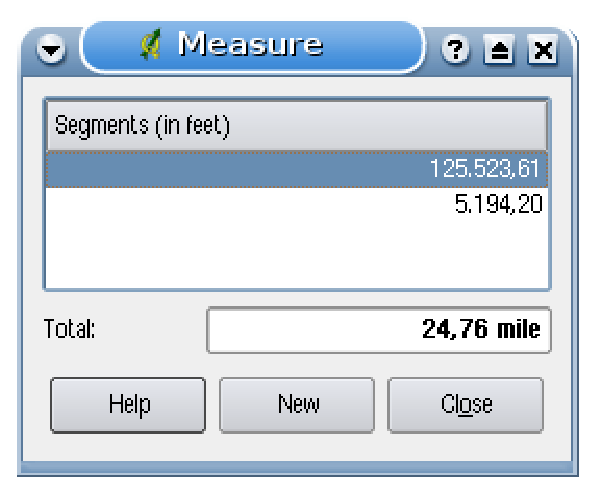
\includegraphics[clip=true, width=0.3\textwidth]{measure_line}}
     \hspace{0.33cm}
   \subfloat[Calcola l'area]{\label{subfig:measure_area}\includegraphics[clip=true, width=0.3\textwidth]{measure_area}}
     \hspace{0.33cm}
   \subfloat[Misura angoli]{\label{subfig:measure_angle}\includegraphics[clip=true, width=0.3\textwidth]{measure_angle}}
   \caption{Strumenti di misura in azione \nixcaption} \label{fig:measure}
\end{figure}

\section{Selezionare e deselezionare elementi}\label{sec:selection}

QGIS fornisce diversi strumenti per la selezione di elementi nella vista mappa.
Per selezionare uno o più elementi cliccare  
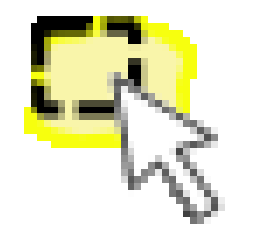
\includegraphics[width=0.7cm]{mActionSelect} e scegliere lo strumento di interesse:

\begin{description}
\item 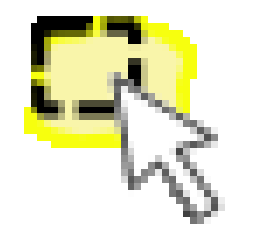
\includegraphics[width=0.5cm]{mActionSelect} Seleziona il singolo elemento
\item \includegraphics[width=0.5cm]{mActionSelectRectangle} Seleziona elementi con un rettangolo
\item \includegraphics[width=0.5cm]{mActionSelectPolygon} Seleziona elementi con un poligono
\item \includegraphics[width=0.5cm]{mActionSelectFreehand} Seleziona elementi a mano libera
\item \includegraphics[width=0.5cm]{mActionSelectRadius} Seleziona elementi con un cerchio
\end{description} 

Per deselezionare tutti gli elementi selezionati cliccare su \includegraphics[width=0.7cm]{mActionDeselectAll}.

\section{Progetti}\label{sec:projects}\index{progetti}

Lo stato di una sessione QGIS è considerato un progetto. 
È possibile lavorare su un progetto alla volta. Le impostazioni possono essere definite 
per ogni singolo progetto oppure di default per tutti i nuovi progetti (Sezione \ref{subsec:gui_options}). 
Lo stato della sessione corrente può essere salvato
in un progetto usando la voce di menu \mainmenuopt{File}\arrow
\dropmenuopttwo{mActionFileSave}{Salva progetto}
o \mainmenuopt{File} \arrow \dropmenuopttwo{mActionFileSaveAs}{Salva progetto con
nome}.

Per caricare progetti salvati usare \mainmenuopt{File} \arrow
\dropmenuopttwo{mActionFileOpen}{Apri progetto}
o \mainmenuopt{File} \arrow \dropmenuopt{Apri progetti recenti}.
Se si vuole eliminare la sessione corrente e ricominciare da zero, scegliere
\mainmenuopt{File} \arrow \dropmenuopttwo{mActionFileNew}{Nuovo progetto}.
Ognuna di queste voci di menu chiederà se si vuole salvare la sessione
corrente qualora fossero occorsi cambiamenti rispetto all'ultima volta in cui la stessa è
stata aperta o salvata.

Le informazioni salvate nel file di progetto includono:

\begin{itemize}
\item Layers aggiunti
\item Proprietà dei layer, inclusa la loro rappresentazione grafica
\item Proiezione usata per la vista mappa
\item Ultima estensione della vista (scala e inquadramento)
\end{itemize}

Il file di progetto è salvato in formato XML, così da poter essere editato
esternamente a QGIS con qualunque editor, se si conosce la sintassi. Il formato
del file di progetto è stato modificato parecchie volte rispetto a quello
delle precedenti versioni di QGIS, di conseguenza file di progetto salvati con
precedenti versioni di QGIS potrebbero non funzionare più correttamente. Si
può essere avvertiti preventivamente di ciò selezionando dalla scheda
\tab{Generale} nel menu \mainmenuopt{Impostazioni} \arrow \dropmenuopt{Opzioni}: 

\checkbox{Richiedi di salvare i cambiamenti di progetto se necessario} \\
\checkbox{Avvisa quando viene aperto un file di progetto salvato con una vecchia versione di QGIS}.

\minisec{Proprietà progetto}
Nella finestra delle proprietà del progetto (sotto \nix{\mainmenuopt{File} \arrow
\dropmenuopt{Proprietà progetto}} o \win{\mainmenuopt{Impostazioni} \arrow
\dropmenuopt{Proprietà progetto}} possono essere impostate opzioni specifiche del progetto. Queste
includono:

\begin{itemize}
\item Nella scheda \tab{Generale} il titolo del progetto, il colore di selezione e dello sfondo, le unità di misura e l'opzione per salvare i percorsi relativi ai layer. È possibile impostare le unità di misura (usato solo quando la riproiezione è disabilitata) e la precisione per le cifre decimali. 
\item La scheda \tab{Sistema di riferimento (SR)} permette di scegliere il sistema di proiezione delle coordinate e di abilitare la riproiezione al volo dei layer vettoriali quando vengono visualizzati layer con differenti SR.
\item La scheda \tab{Layer interrogabili} permette di definire i layer che risponderanno allo strumento di interrogazione. (Vedere il paragrafo Strumenti mappa nella sezione \ref{subsec:gui_options} per abilitare l'interrogazione di layer multipli.)
\item La scheda \tab{Server WMS} permette di definire le informazioni del Service Capabilities, l'Estensione pubblicata e le Restrizioni dei sistemi di coordinate del mapserver QGIS. Attivando \checkbox{Aggiungi geometria WKT alle informazioni di risposta dell'oggetto} il layer WMS risulterà interrogabile.
\end{itemize}

\section{Output}\label{sec:output}\index{output!salva come immagine!gestore di stampe}
Ci sono diversi modi per generare file di output da una sessione QGIS.
Il primo è stato descritto alla Sezione \ref{sec:projects} e consiste nel
salvataggio su file di progetto. 
Altri modi di produrre file di output sono ad esempio:
\begin{itemize}
\item L'opzione di menu \dropmenuopttwo{mActionSaveMapAsImage}{Salva come
immagine} permette di salvare la vista mappa come immagine in formato PNG o JPG: insieme all'immagine viene salvato anche un file di georeferenziazione (world file) con estensione rispettivamente PNGW o JPGW.
\item L'opzione di menu \dropmenuopttwo{mActionNewComposer}{Nuova composizione di stampa} apre una finestra di dialogo dove è possibile impaginare e stampare la vista mappa (Sezione~\ref{label_printcomposer}).
\end{itemize}

\section{Opzioni dell'interfaccia grafica (GUI)}\label{subsec:gui_options}

\includegraphics[width=0.7cm,clip=true]{mActionOptions} Alcune opzioni di base per QGIS 
possono essere impostate nella finestra \dialog{Opzioni}. Selezionare la 
voce di menu \mainmenuopt{Impostazioni} \arrow \dropmenuopttwo{mActionOptions}{Opzioni}. Le schede nelle quali possono essere regolate le opzioni sono:

\minisec{Generale}

\begin{itemize}
\item \checkbox{Richiedi di salvare i cambiamenti di progetto se necessario}
\item \checkbox{Avvisa quando viene aperto un file di progetto salvato con una vecchia versione di QGIS}
\item Colore della selezione
\item Colore di sfondo
\item Tema delle icone (scelta tra default e gis)
\item Dimensione delle icone (scelta tra 16, 24 e 32)
\item Azione eseguita in legenda sul comando doppio-click (scelta tra "Apri proprietà del layer" e "Apri tabella degli attributi")
\item \checkbox{Rendi maiuscoli i nomi dei layer nella legenda}
\item \checkbox{Visualizza i nomi degli attributi della classificazione nella legenda}
\item \checkbox{Crea le icone raster nella legenda}
\item \checkbox{Nascondi lo splash screen all'avvio}
\item \checkbox{Mostra suggerimenti all'avvio}
\item \checkbox{Apri i risultati di un'interrogazione in una finestra agganciata (richiede il riavvio di QGIS)}
\item \checkbox{Apri la tabella attributi in una finestra agganciata(richiede il riavvio di QGIS)}
\item \checkbox{Aggiungi un layer PostGIS con un doppio click e seleziona la modalità  estesa}
\item \checkbox{Aggiungi nuovi layer al gruppo selezionato}
\item Comportamento della tabella attributi (scelta tra Mostra tutti gli elementi, Mostra gli elementi selezionati, Mostra gli elementi sulla mappa corrente)
\item Mostra i valori NULL come 
\item Percorsi per cercare ulteriori librerie plugin C++. 
\end{itemize}

\minisec{Visualizzazione in corso}

\begin{itemize}
\item \checkbox{Per impostazione predefinita i nuovi layer aggiunti alla mappa vengono visualizzati subito}
\item Numero di geometrie da disegnare prima di aggiornare lo schermo.
\item \checkbox{Usa il caching del disegno quando possibile per velocizzare la visualizzazione}
\item \checkbox{Rendi le linee meno irregolari a spese delle prestazioni}
\item \checkbox{Risolvi problemi con i poligoni riempiti non correttamente}
\item \checkbox{Utilizza la nuova generazione di simboli per la visualizzazione}
\item Percorso(i) dove cercare simboli SVG (Scalable Vector Graphics) 
\end{itemize}

È possibile definire se salvare i percorsi alle texture svg in modalità assoluta o relativa nella scheda \tab{Generale} 
del menu \mainmenuopt{Impostazioni} \arrow \dropmenuopttwo{mActionOptions}{Proprietà progetto}.

\minisec{Strumenti mappa}

\begin{itemize}
\item L'impostazione Modalità determina quali layer saranno mostrati attraverso
lo strumento 'Informazioni elementi'. Passando a \usertext{Top down} o \usertext{Il primo attivo} invece di  
\usertext{Layer in uso} gli attributi di tutti i layer selezionabili 
(Si veda la Sezione Proprietà progetto in: \ref{sec:projects} sulle modalità di impostazione dei layer selezionabili) 
saranno visibili tramite lo strumento Informazioni elementi.
\item \checkbox{Apri il modulo degli elementi se viene identificato un un singolo elemento}
\item Specificare il raggio di ricerca come percentuale della larghezze della mappa.
\item Ellissoide per calcoli di distanza
\item Colore elastico
\item Posizioni decimali
\item \checkbox{Mantieni le unità di base}
\item \radiobuttonon{Unità di misura preferita (Metri o Piedi)}
\item \radiobuttonon{Unità preferita per gli angoli (Gradi, Radianti o Gradi Decimali)}
\item Azione della rotellina del mouse (Zoom, Zoom e centramento, Zoom al cursore del mouse, Niente)
\item Fattore di zoom
\end{itemize}

\minisec{Sovrapposizioni}

\begin{itemize}
\item Definizione dell'algoritmo di posizionamento delle etichette (scelta tra Punto centrale, Catena, Catena tabu popmusic, Tabu popmusic, Catena popmusic)
\end{itemize}

\minisec{Digitalizzazione}

\begin{itemize}
\item Colore e spessore della linea
\item Modalità di snap predefinita (al vertice, al segmento o entrambe)
\item Tolleranza di snapping predefinita in unità di mappa o in pixel
\item Raggio di ricerca per le modifiche dei vertici in unità di mappa o in pixel
\item \checkbox{Utilizza indicatori solo per le geometrie selezionate}
\item Stile indicatore (croce, cerchio semitrasparente o nessuno) e della dimensione per gli indicatori dei vertici 
\item \checkbox{Ripeti i valori degli attributi usati per ultimi}
\item \checkbox{Non aprire la finestra degli attributi dopo la creazione di ogni geometria}
\end{itemize}

\minisec{SR}

La scheda SR è divisa in due aree. La prima permette di impostare il SR predefinito per i nuovi progetti: 

\begin{itemize}
\item Inizia un nuovo progetto sempre con questo SR.
\item \checkbox{Effettua sempre la riproiezione al volo}
\end{itemize}

La seconda area permette di definire cosa accade quando un nuovo layer viene creato o quando viene caricato un layer senza SR.
\begin{itemize}
\item \radiobuttonoff{Richiedi SR}
\item \radiobuttonoff{Usa il SR del progetto}
\item \radiobuttonon{Utilizza come predefinito il SR visualizzato sotto}
\end{itemize}

\minisec{Lingua}

\begin{itemize}
\item \checkbox{Sovrascrivi lingua in uso}
\item Informazioni sulla lingua correntemente impostata nel sistema
\end{itemize}

\minisec{Rete}

\begin{figure}[ht]
   \centering
   \includegraphics[clip=true, width=14cm]{proxy-settings}
   \caption{Impostazione proxy in \qg \nixcaption}
   \label{fig:proxy-settings}
\end{figure}

\begin{itemize}
\item \checkbox{Utilizza un proxy per l'accesso web}, definizione di host,porta, utente e password.
\item Definizione del \dropmenuopt{Tipo proxy} 
\begin{itemize}
  \item \dropmenuopt{Default Proxy}: Il proxy è determinato sulla base delle impostazioni in uso del proxy dell'applicazione
  \item \dropmenuopt{Socks5Proxy}: Proxy generico per ogni tipo di connessione. Supporta TCP, UDP, associazione a una porta (connessione in entrata) e autenticazione.
  \item \dropmenuopt{HttpProxy}: Realizzato usando il comando "CONNECT", supporta solamente connessioni TCP in uscita; supporta l'autenticatione.
  \item \dropmenuopt{HttpCachingProxy}: Realizzato usando normali comandi HTTP, è utile solamente nel contesto di richieste HTTP.
  \item \dropmenuopt{FtpCachingProxy}: Realizzato usando un proxy FTP, è utile solamente nel contesto di richieste FTP.
 \end{itemize}
\item Impostazioni della cache (cartella e dimensione)
\item Indirizzo di ricerca WMS (Quello predefinito è \url{http://geopole.org/wms/search?search=\%1\&type=rss}
\item Timeout per le richieste di rete in ms - predefinito 60000
\end{itemize}

Si possono escludere alcuni URL aggiungendole nella casella di testo al di sotto delle impostazioni del proxy 
(Figura \ref{fig:proxy-settings}) premendo il pulsante \button{Aggiungi}. In seguito 
fare doppio click nel campo URL appena creato e inserire l'URL che si desidera
escludere dall'utilizzo del proxy. Ovviamente il pulsante \button{Rimuovi} elimina l'elemento selezionato.

Per informazioni più dettagliate sulle diverse impostazioni del proxy,
si prega di fare riferimento al manuale della documentazione delle librerie QT su
\url{http://doc.trolltech.com/4.5/qnetworkproxy.html#ProxyType-enum}.

\begin{Tip} \caption{\textsc{Utilizzo dei proxy}}
L'utilizzo dei proxy può a volte essere complicato. E' utile testare i tipi di proxy succitati e controllare il loro funzionamento nel vostro caso specifico.
\end{Tip}

Queste opzioni possono essere modificate in funzione delle proprie esigenze. Alcuni cambiamenti potrebbero richiedere il riavvio di QGIS prima di essere attivi.

\begin{itemize}
\item \nix{Le impostazioni sono salvate in un file di testo: \$HOME/.config/QuantumGIS/qgis.conf}
\item \osx{Le impostazioni vengono collocate in: \$HOME/Library/Preferences/org.qgis.qgis.plist}
\item \win{Le impostazioni vengono inserite nel registro di sistema alla voce:}
\begin{verbatim}
\\HKEY\CURRENT\USER\Software\QuantumGIS\qgis
\end{verbatim}
\end{itemize}

\section{Note testuali}\label{sec:annotations}
\index{note}
\index{note testuali|\vedi {note}}

Lo strumento \includegraphics[width=0.7cm,clip=true]{mActionTextAnnotation} note nella barra degli attributi permette di 
posizionare del testo formattato sulla vista mappa di QGIS. Scegliere lo strumento note e cliccare nella vista mappa.

\begin{figure}[ht]
   \centering
   \includegraphics[clip=true, width=12cm]{annotation}
   \caption{Finestra di dialogo delle note \nixcaption}
   \label{fig:annotation}
\end{figure}

Facendo doppio-click sull'elemento aggiunto sulla mappa dallo strumento note si ha accesso ad una finestra di dialogo con varie opzioni. C'è un editor di testo semplificato per l'inserimento del testo formattato; è possibile scegliere se vincolare il testo alla mappa o solo allo schermo. 
Il testo può essere spostato secondo le proprie esigenze tramite lo strumento \includegraphics[width=0.7cm,clip=true]{mActionAnnotation} {Muovi nota}.

\subsection{Nota con modulo}\index{note}
\index{nota con modulo|\vedi {note}}

È possibile creare moduli note personalizzati. Lo strumento \includegraphics[width=0.7cm,clip=true]{mActionFormAnnotation} Note con modulo è utile per visualizzare gli attributi di un layer vettoriale in un modulo personalizzato qt designer (Figura \ref{fig:custom-annotations}). 
È simile alla finestra dello strumento 'Informazioni elementi', ma il tutto viene mostrato in una nota. Si veda il blog \url{http://blog.qgis.org/node/143} per maggiori dettagli.

\begin{figure}[ht]
   \centering
   \includegraphics[clip=true, width=10cm]{custom_annotation}
   \caption{Modulo nota qt designer personalizzato \nixcaption}
   \label{fig:custom-annotations}
\end{figure}

\textbf{Nota:} Premendo Ctrl-T con uno strumento nota attivo (Nota testuale, Nota con modulo, Muovi nota) lo stato di visualizzazione delle note si inverte: se sono visibili diventano invisibili e viceversa.

\newpage

\section{Segnalibri geospaziali}\label{sec:bookmarks}
\index{segnalibri}
\index{segnalibri geospaziali|\vedi {segnalibri}}

I segnalibri geospaziali consentono di "memorizzare" una posizione geografica alla quale ritornare in un secondo momento.

\subsection{Creazione di un segnalibro}
Per creare un segnalibro:
\begin{enumerate}
\item Usare lo zoom o muovere la mappa all'estensione d'interesse.
\item Selezionare la voce di menu \mainmenuopt{Visualizza} \arrow
\dropmenuopt{Nuovo segnalibro} o premere \keystroke{Ctrl-B}.
\item Inserire un nome descrittivo per il segnalibro (fino a 255 caratteri).
\item Cliccare su \button{OK} per aggiungere il segnalibro o \button{Cancel}
per uscire senza aggiungere il segnalibro.
\end{enumerate}

Si noti che è possibile avere più di un segnalibro con lo stesso nome.

\subsection{Uso e gestione dei segnalibri}
Per usare o gestire i segnalibri, selezionare la voce di menu
\mainmenuopt{Visualizza} \arrow \dropmenuopt{Mostra segnalibri}.
La finestra \dialog{Segnalibri geospaziali} consente di usare lo zoom a un
segnalibro o di eliminarne uno.
Non è possibile editare il nome o le coordinate di un segnalibro.

\subsection{Zoom a un segnalibro}
Dalla finestra \dialog{Segnalibri geospaziali}, selezionare il
segnalibro desiderato cliccando su di esso, quindi cliccare su \button{Zoom a}.
Si può usare lo zoom su un segnalibro anche facendo doppio click su di esso.

\subsection{Cancellare un segnalibro}
Per cancellare un segnalibro dalla finestra \dialog{Segnalibri geospaziali},
cliccare su di esso e poi sul pulsante \button{Elimina}.
Confermare la scelta cliccando su \button{OK} o annullare l'eliminazione
cliccando su \button{Cancel}.

\section{Tracciamento GPS in tempo reale}\label{sec:gpstracking}

Per attivare tale funzione selezionare la voce di menu \mainmenuopt{Visualizza} \arrow \dropmenuopt{Tracciamento GPS in tempo reale}.
Apparirà una nuova finestra ancorata nella parte sinistra della vista mappa. La finestra presenta quattro schermate differenti
(Figura \ref{fig:gpstrack_live} e Figura \ref{fig:gpstrack_options}).

\begin{description}
 \item[(a)] 
\includegraphics[width=0.5cm,clip=true]{mActionToggleEditing}
Coordinate della posizione GPS ed inserimento vertici e geometrie
 \item[(b)] \includegraphics[width=0.5cm,clip=true]{gpstrack_barchart}
Forza del segnale GPS delle connessioni ai satelliti
 \item[(c)] \includegraphics[width=0.5cm,clip=true]{gpstrack_polarchart}
Diagramma polare del GPS con numero e posizione dei satelliti
 \item[(d)] 
\includegraphics[width=0.5cm,clip=true]{mActionOptions}
Opzioni del GPS (Figura \ref{fig:gpstrack_options}).
\end{description}

Collegato un ricevitore GPS al computer (deve essere supportato dal sistema operativo), un semplice click su \button{Connetti} 
connette il GPS a QGIS. Un secondo click (ora \button{Disconnetti}) disconnette il ricevitore GPS dal computer.
Per il sistema operativo GNU/Linux l'integrazione del supporto gpsd permette la connessione alla maggior parte dei ricevitori
GPS. È comunque necessario configurare adeguatamente gpsd.

[ IMPORTANTE ]: Se si vuole memorizzare la propria posizione rispetto alla vista mappa bisogna creare
preventivamente un nuovo file vettoriale ed impostarlo come modificabile: in tal modo la traccia GPS verrà
memorizzata come vettore.

\begin{figure}[ht]
\centering
   \subfloat[Coordinate posizione] {\label{subfig:gpstrack_main}\includegraphics[clip=true, width=0.3\textwidth]{gpstrack_main}}
     \hspace{0.33cm}
   \subfloat[Forza segnale GPS]{\label{subfig:gpstrack_stren}\includegraphics[clip=true, width=0.3\textwidth]{gpstrack_stren}}
     \hspace{0.33cm}
   \subfloat[Diagramma polare GPS]{\label{subfig:gpstrack_polar}\includegraphics[clip=true, width=0.3\textwidth]{gpstrack_polar}}
\caption{Tracciamento GPS in tempo reale \nixcaption} \label{fig:gpstrack_live}
\end{figure}

\begin{figure}[ht]
   \centering
   \includegraphics[clip=true, width=4cm]{gpstrack_options}
   \caption{Finestra opzioni GPS \nixcaption}
   \label{fig:gpstrack_options}
\end{figure}

\subsection{Coordinate della posizione}

\includegraphics[width=0.5cm,clip=true]{mActionToggleEditing} Le coordinate 
della posizione sono espresse in latitudine, longitudine ed elevazione 
come mostrato in Figura \ref{subfig:gpstrack_main}
(si presuppone che il GPS stia ricevendo segnale dai satelliti). 

\subsection{Forza segnale GPS}
\includegraphics[width=0.5cm,clip=true]{gpstrack_barchart} La schermata 
mostra la forza del segnale che si sta ricevendo dai satelliti 
(Figura \ref{subfig:gpstrack_stren}).

\subsection{Diagramma polare GPS}
\includegraphics[width=0.5cm,clip=true]{gpstrack_polarchart} Il diagramma 
polare mostra la posizione dei satelliti cui si è connessi 
(Figura \ref{subfig:gpstrack_polar}). Viene inoltre mostrato 
l'ID (numero identificativo) dei singoli satelliti.

\subsection{Opzioni GPS}

\includegraphics[width=0.5cm,clip=true]{mActionOptions} In caso di problemi 
di connessione disabilitare il riconoscimento automatico del 
GPS \radiobuttonon{Individuazione automatica} ed utilizzare  
\radiobuttonon{Usa il percorso e la porta indicata} per inserire manualmente 
il percorso e la porta cui è connesso il ricevitore GPS: quindi cliccare su
\button{Connetti} per reinizializzare la connessione.

Con \slider{Dimensione cursore del GPS} è possibile gestire la dimensione del 
cursore del GPS nella vista mappa. 
Attivando \radiobuttonon{Aggiungi vertici automaticamente} la traccia GPS 
verrà memorizzata nel layer vettoriale attivo (se lo stesso è in modalità di modifica)

Con 'Centra la mappa sulla posizione GPS' è possibile decidere le modalità di 
aggiornamento della vista mappa qualora le coordinate memorizzate iniziano 
ad essere esterne all'estensione della vista stessa o comunque in seguito ad un
qualche cambiamento.

In Traccia è possibile impostare colore e spessore della traccia GPS.

Se si vuole impostare una geometria manualmente, tornare a 

\includegraphics[width=0.5cm,clip=true]{mActionToggleEditing} 'Coordinate della posizione'
e cliccare \button{Aggiungi geometria}.

\FloatBarrier
